\newrobustcmd*{\square}[1]{\tikz{\filldraw[draw=#1,fill=#1] (0,0)
rectangle (0.2cm,0.2cm);}}

\newrobustcmd*{\mycircle}[1]{\tikz{\filldraw[draw=#1,fill=#1] (0,0) circle [radius=0.1cm];}}

\newrobustcmd*{\mytriangle}[1]{\tikz{\filldraw[draw=#1,fill=#1] (0,0) --
(0.2cm,0) -- (0.1cm,0.2cm);}}

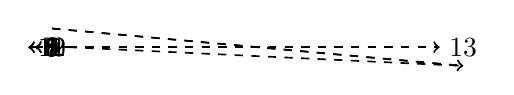
\begin{tikzpicture}[sibling distance=20pt]
\tikzset{level distance=30pt}
\Tree[.\node(0){0}; [.\node(1){1}; [.\node(2){2}; \mytriangle{red}A ]
               [.\node(3){3}; \mytriangle{red}B ]]
          [.\node(4){4}; [.\node(5){5}; \mytriangle{red}C ]
                [.\node(6){6};
                [.\node(7){7}; [.\node(8){8}; \mytriangle{red}D ][.\node(9){9}; \mytriangle{red}E ]]
                [.\node(10){10}; [.\node(11){11}; \mytriangle{red}F ]
                [.\node(12){12}; \mytriangle{red}G ]]]]]
\node [anchor=base, right=14em]  (13) {13};
\draw[semithick,dashed,->] (1.east) to (4.west);
\draw[semithick,dashed,->] (2.east) to (3.west);
\draw[semithick,dashed,->] (3.east) to (4.west);
\draw[semithick,dashed,->] (5.east) to (6.west);
\draw[semithick,dashed,->] (7.east) to (10.west);
\draw[semithick,dashed,->] (8.east) to (9.west);
\draw[semithick,dashed,->] (7.east) to (10.west);
\draw[semithick,dashed,->] (9.east) to (10.west);
\draw[semithick,dashed,->] (11.east) to (12.west);
\draw[semithick,dashed,->] (0.east) to (13.west);
\draw[semithick,dashed,->] (4.east) to (13.west);
\draw[semithick,dashed,->] (6.east) to (13.south);
\draw[semithick,dashed,->] (10.north) to (13.south);
\draw[semithick,dashed,->] (12.north) to (13.south);

\end{tikzpicture}
